\documentclass[a4paper,10pt,notitlepage]{article}
\usepackage{ctex,geometry,graphicx,tikz,setspace,paralist,fancyhdr,caption}
\geometry{
	left=1.5cm,
	right=1.5cm,
	top=1.4cm,
	bottom=2cm,}
\newcommand{\rec}{
	\begin{tikzpicture}[remember picture,overlay]
		% 绘制边框
		\draw[line width=1.2pt] ([xshift=0.5cm,yshift=0.5cm] current page.south west) rectangle ([xshift=-0.5cm,yshift=-0.8cm] current page.north east);
	\end{tikzpicture}
	
}
\pagestyle{fancy}
\fancyhf{}
\fancyhead[C]{\rec}  % 在页眉中绘制图形
\fancyhead[L]{附录}
\fancyhead[R]{实验七 \quad 积分与微分电路}
\fancyfoot[C]{\thepage}
\begin{document}
	\large
	\onehalfspacing
	\begin{figure}[h]
		\raggedright
		
\includegraphics{1.png}
	\end{figure}
	\centering
	{\Huge\textbf{模电实验报告}\par}
	\vspace{0.2cm}
	{\huge{实验内容:积分与微分电路}\par}
	\raggedright
	\vspace{0.3cm}
	\begin{centering}
		{\large 院系:电子与信息工程学院\hfill 学号:22309080\hfill 审批:\hspace{2cm} \par
			专业:通信工程\hfill 实验人:梁倍铭\hfill 日期:2023年11月22日 \par}
	\end{centering}
	\vspace{0.3cm}
	\section*{一、积分电路}
	\begin{enumerate}
	\item 仿真波形如图
	\begin{figure}[h]
		\centering
		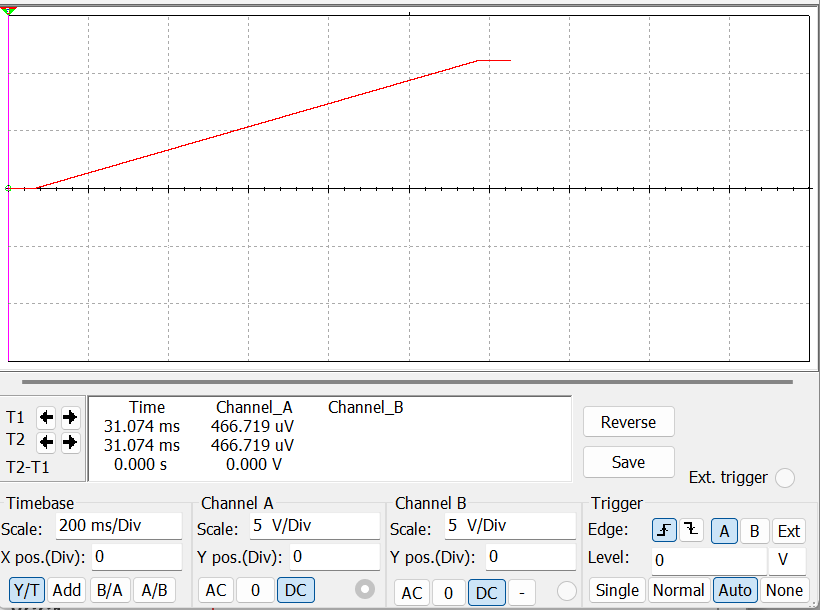
\includegraphics[width=0.3\textwidth]{2.png}
		\caption*{图1}
	\end{figure}
	\item 饱和输出电压及有效积分时间
	\begin{table}[h]
		\centering
		\begin{tabular}{|c|c|c|}
			\hline
			& 饱和输出电压(V) & 有效积分时间(s) \\
			\hline
			仿真 & 11.098 & 1.101 \\
			\hline 
			实验 & \qquad & \qquad \\
			\hline
		\end{tabular}
		\caption*{表1}
	\end{table}
	\item 使图7-1 中积分电容改为0.1μ,断开K1,Vi 分别输入100Hz 幅值为2V 方
	波正弦波信号,观察Vi 和Vo 大小及相位关系,并记录波形。
	\newpage
	\begin{figure}[h]
		\centering
		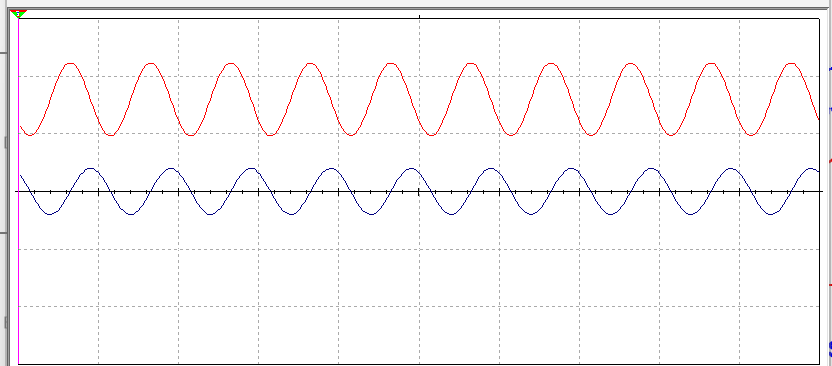
\includegraphics[width=0.3\textwidth]{3.png}
		\caption*{图2}
	\end{figure}
\end{enumerate}
\section*{二、微分电路}
\begin{enumerate}
	\item 输入有效值为lV,f =160Hz 三角波(正弦波)信号,用示波器观察Vi 与Vo
	波形并测量输出电压。
	\begin{figure}[h]
		\centering
		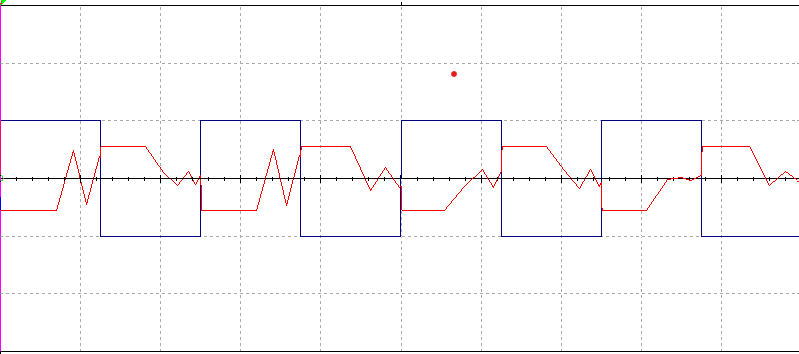
\includegraphics[width=0.3\textwidth]{4.png}
		\caption*{图3}
	\end{figure}
	\item 改变三角波(正弦波)频率(20HZ~400HZ),观察Vi 与Vo 的相位、幅值变化
	情况并记录。
	\begin{table}[h]
		\centering
		\begin{tabular}{|c|c|c|c|c|c|c|c|}
			\hline
			频率(Hz) & 20 & 50 & 100 & 150 & 200 & 300 & 400 \\
			\hline
			仿真幅值 & 0.277 & 0.7 & 1.38 & 2.08 & 2.775 & 4.16 & 5.55\\
			\hline 
			实验幅值 & \qquad & \qquad & \qquad & \qquad & \qquad & \qquad &\qquad \\
			\hline
		\end{tabular}
		\caption*{表2 幅值}
	\end{table}
	\item 输入V= ±5V,f =200Hz 的方波信号,用示波器观察Vo 波形,按上述步骤重
	复实验。
	\begin{figure}[h]
		\centering
		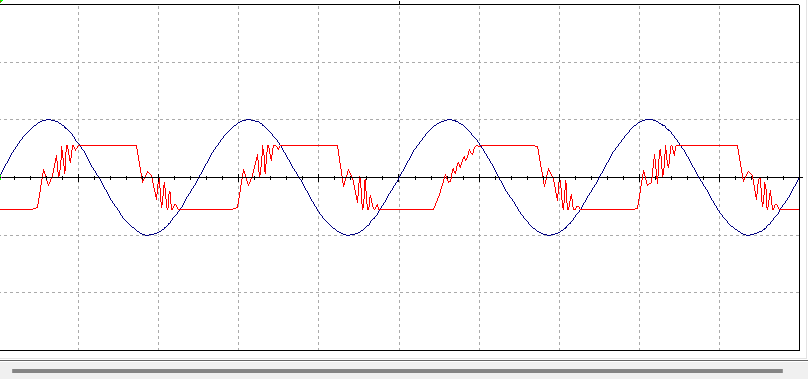
\includegraphics[width=0.4\textwidth]{5.png}
		\caption*{图4}
		\end{figure}
\end{enumerate}
\end{document}